%
%% 2019 07 04 Ph. G. Freimann
%%

\section{Lineare Gleichungen\TALS{ I}}\index{Gleichungen!lineare}\index{lineare Gleichung}\label{gleichungen_lineare}
\sectuntertitel{... weil keine zwei Dinge gleicher sein
  können.\footnote{\textit{Robert Recorde} (1557; \textit{Der
      Wetzstein des Wissens}) über das
    Gleichheitszeichen\index{Gleichheitszeichen} als zwei Parallele:
    «... weil keine zwei Dinge gleicher sein können.»}}

%%\TALSTadBFWA{81}{2.2}
%%%%%%%%%%%%%%%%%%%%%%%%%%%%%%%%%%%%%%%%%%%%%%%%%%%%%%%%%%%%%%%%%%%%%%%%%%%%%%%%%
\subsection*{Lernziele}

\begin{itemize}
\item Lineare Gleichungen
\item Äquivalenzumformung / Lösungsmenge
\item Grundform (GF) linearer Gleichungen
\item Textaufgaben, die zu Gleichungen\index{Textgleichungen}\TALS{
  (ev. mit Parametern)} führen.
\TALS{\item Einsatz des Taschenrechners}
\end{itemize}

\TadBMTA{115}{8}

\newpage

\TRAINER{\GESO{Bem. «Lineare Gleichungen erst mal ohne ohne Parameter»}}
\noTRAINER{\vspace{10mm}}


\begin{beispiel}{Einstiegsbeispiel}{}

  $2x-7+3x = 5x-6-\frac{x}{2}$ 

\TNT{6.4}{  \begin{tabular}{ll}
    $2x-7+3x = 5x-6-\frac{x}{2}$                      & $| \cdot{} 2$\\
    $(2x-7+3x)\cdot{} 2 = (5x-6-\frac{x}{2})\cdot{}2$ & $| TU$\\
    $4x-14+6x = 10x-12-x$ & $| +x$\\
    $5x-14+6x = 10x-12$ & $| $ TU $ = $ Termumformung\\
    $11x-14 = 10x-12$ & $|-10x$\\
    $x-14 = -12$ & $|+14$\\
    $x = 2$ & \\
    \end{tabular}

  Probe: Setze $\color{red}x=2$ in die Originalgleichung ein:

  $$2\cdot{}{\color{red}2}-7+3\cdot{}{\color{red}2} = 5\cdot{}{\color{red}2}-6-\frac{{\color{red}2}}{2}$$
  $$4-7+6 = 10 -6 -1 \textrm{ \color{green} OK!}$$
  }%% END TNT
\end{beispiel}
\newpage

\index{Lineare Gleichung!Grundform}\index{Grundform!lineare Gleichung}
\begin{definition}{Lineare Gleichung}{definition_lineare_gleichung}
  Bei einer \textbf{linearen Gleichung} kommt die Gesuchte in der
  1. Potenz vor; \zB $x (= x^1)$.
\end{definition}

\begin{definition}{Grundform}{}\index{Grundform!lineare Gleichung}\index{Lineare Gleichung!Grundform}
  \textbf{Grundform}\index{Grundform!lineare Gleichung}:\\
  $$ax+b=0 \textrm{ mit } a,b\in\mathbb{R}, a\ne 0$$
  
  \end{definition}

\begin{gesetz}{Lösungsformel}{}
 Lösung der linearen Gleichung in der Grundform

 $$ax+b=0$$
 \TNT{2}{$$ax=-b$$\vspace{10mm}}
  $$x = \frac{-b}a$$
  
\end{gesetz}

\newpage
\textbf{Grundform}\index{Grundform!lineare Gleichung}\\

\begin{beispiel}{Grundform}{beispiel_lineare_gleichung_grundform}
  Bringen Sie die folgende lineare Gleichung auf die Grundform:
  $$2x-10 = -3x\TRAINER{\,\,\,| +3x}$$

  Grundform: $\LoesungsRaum{5x-10} = 0$

  $a = \LoesungsRaum{5}$

  $b = \LoesungsRaum{-10}$

  und somit

  \LARGE{$x=\frac{-(\noTRAINER{\,\,\,\,\,\,}\TRAINER{-10})}{\noTRAINER{\,\,\,\,\,\,\,}\TRAINER{5}}
    = \LoesungsRaum{2}$}

\end{beispiel}


\begin{beispiel}{Lineare Gleichung}{beispiel_lineare_gleichung_3x7}
  Die Gleichung $3x=-7$ ist äquivalent zur Grundform $3x+7=0$ und somit ist die Lösung $\LoesungsRaum{\frac{-7}{3}}$
  \end{beispiel}

\begin{beispiel}{Lineare Gleichung}{beispiel_lineare_gleichung_5x8}
  Die Gleichung $-5x=8$ ist äquivalent zur Grundform $-5x-8=0$ und somit ist die Lösung $\LoesungsRaum{\frac{8}{-5}}$
\end{beispiel}
\newpage

\TALS{\input{allg/gleichungen/GraphischeInterpretationLinearerGleichungen}}
  
\newpage
\subsection{Äquivalenzumformungen}\index{Aquivalenzumformungene@Äquivalenzumformungen}
Äqui... = Gleich...; ...valenz = ...wertig

\TadBMTA{111ff}{7.2}
%%\TALS{S. \cite{frommenwiler17alg} Seite 79 (Äquivalenz von Aussageformen)}
%%\TALS{S. \cite{frommenwiler17alg} Seite 80 (Liste der Äquivalenzumformungen)}
%%\GESO{S. \cite{marthaler21alg} Seite 111 (Liste der Äquivalenzumformungen)}


\textbf{Äquivalenzumformungen sind}

\begin{tabular}{lp{6cm}p{8cm}}\hline\\%%
Umformung   & Beschreibung  & Beispiel \\\hline
$| $ TU      & Termumformung & {\raggedright Beispiel: Links des Gleichheitszeichens $a$ ausklammern; gilt , sofern sich die Definitionsmenge des Terms nicht ändert!}\\
$| $ $+ T(x)$  & Term beidseitig addieren. & $| \color{ForestGreen}+4$, $| \color{ForestGreen}+\sqrt{x}$, $| \color{ForestGreen}+8\cdot{}x^2$\\
$| $ $- T(x)$  & Term beidseitig subtrahieren. & $| \color{ForestGreen}-6$, $|\color{ForestGreen}-x^3$, $|\color{ForestGreen} -5x$\\
$| $ $\cdot{} T$  & Mit von Null verschiedenem Term $T$ multiplizieren. & $| \color{ForestGreen}\cdot{} 3$, $|\color{ForestGreen}\cdot{}(2+\sqrt{5})$, $|\color{ForestGreen}\cdot{}a^2; a\ne 0$\\
$| $ $: T$  & Durch von Null verschiedenem Term $T$ dividieren. & $| \color{ForestGreen}: 6$, $|\color{ForestGreen}: \frac{\pi}6$, $|\color{ForestGreen}:\sqrt{b}; b> 0$\\
\end{tabular}

\textbf{keine} Äquivalenzumformungen sind

\begin{tabular}{lp{6cm}>{\raggedright}p{4cm}p{4cm}}\hline\\
Umformung  & Beschreibung &Lösungen können... & Beispiel\\\hline
%%$| $ TU & Termumformung & ... ändern & {| \color{red} TU $(x+1)$ kürzen}\\
$| $ potenzieren  & Beide Seiten potenzieren & \LoesungsRaum{...hinzukommen.}&$| \color{red}\Box{}^6$\\
$| $ radizieren & Auf beiden Seiten die Wurzel ziehen& \LoesungsRaum{...verschwinden.}&$| \color{red}\sqrt[4]{\,}$\\
$| $ $\cdot{}T(x)$  & mit der Unbekannten multiplizieren & \LoesungsRaum{...hinzukommen.}&$| \color{red}\cdot{}(x+4)$, $| \color{red}\cdot{}3x^2$\\
$| $ $:T(x)$  & durch Unbekannte dividieren & \LoesungsRaum{... verschwinden.}&$|
\color{red}:(x-8)$, $| \color{red}:\sqrt{x}$\\

\end{tabular}
\newpage

\subsubsection{Finde Äquivalenzumformungen}
Der folgende Lösungsweg ist definitiv falsch. Irgendwo ist eine Umformung vorgenommen worden, die nicht gültig ist.
Schreiben Sie bei jeder Umformung hin, um welche der oben angegebenen gültigen Äquivalenzumformung es sich handelt. Finden Sie den Fehler:

Im folgenden seien $\pi$ und $a$ als die Kreiszahl $3.14159...$ definiert. Es gilt also $\pi = a$.
\begin{tabular}{lr@{$=$}lp{7cm}}
                  & $a$              & $\pi$               & nach Voraussetzung       \\
$\Longrightarrow$ & $a\cdot a$       & $a\cdot\pi$         & wegen .........................     \\ 
$\Longrightarrow$ & $a^2$            & $a\pi$              & ................................... \\ 
$\Longrightarrow$ & $a^2 + a^2$      & $a\pi + a^2$         & ................................... \\
$\Longrightarrow$ & $2a^2$           & $a\pi + a^2$         & ................................... \\ 
$\Longrightarrow$ & $2a^2-2a\pi$     & $a\pi + a^2 -2a\pi$  & ................................... \\ 
$\Longrightarrow$ & $2a^2-2a\pi$     & $\,\,\,\,\,\,\,\,\,\,\,\,\,\,  a^2 -a\pi$  & ................................... \\ 
$\Longrightarrow$ & $2a^2-2a\pi$     & $a\cdot(a-\pi)$     & ................................... \\ 
$\Longrightarrow$ & $2a\cdot(a-\pi)$ & $a\cdot(a-\pi)$     & ................................... \\ 
$\Longrightarrow$ & $\frac{2a\cdot(a-\pi)}{a-\pi}$ & $\frac{a\cdot(a-\pi)}{a-\pi}$     & \noTRAINER{...................................} \TRAINER{hier wurde durch 0 dividiert, denn $a=\pi$!}\\ 
$\Longrightarrow$ & $2a$             & $\frac{a\cdot(a-\pi)}{a-\pi}$     & \noTRAINER{...................................}\TRAINER{Definitionsbereich durch Termumformung links verändert} \\ 
$\Longrightarrow$ & $2a$             & $a$                 & \noTRAINER{...................................}\TRAINER{Definitionsbereich durch Termumformung rechts verändert} \\ 
$\Longrightarrow$ & $2$              & $1$                 & ........................ \\ 
\end{tabular}
\newpage

\TALS{%%
%% 2019 11 14 Ph. G. Freimann
%%

\subsection{Gleichungen mit CAS lösen (optional)}\index{CAS@Computer Algebra System}\index{Computer Algebra System@CAS}
Damit weniger Fehler geschehen, aber auch, um schneller an Resultate zu gelangen werden in der Praxis Gleichungen fast ausschließlich mit einem Computer-Algebra-System (CAS) gelöst.
Wir wählen eine einfache Gleichung, damit wir a) nicht viel tippen müssen und b) das Resultat auch sofort überprüfen können. Gegeben ist also die folgende Gleichung:

$$3x+1=2x$$

Typischerweise bieten sich die folgenden drei Lösungswege an\footnote{Die drei Verfahren wurden mit dem Rechner ``TI-nspire II-CX CAS'' getestet.}:
\begin{itemize}
\item solve($3x+1=2x$, $x$)
\item $\text{gl1} := 3x+1=2x$\\
  solve($\text{gl1}$, $x$)
  
\item $term1 := 3x+1$\\
  $\text{term2} := 2x$\\
  solve($\text{term1}=\text{term2}$, $x$)\\
  Diese letzte Variante hat den Vorteil, dass wir die Terme leicht als Funktionen in $x$ auffassen können und diese im Graph-Modus sofort anzeigen können:
  \begin{enumerate}
    \item Neue «Page» (1.2) erstellen (+page) als Graph. 
    \item Tippe $f1(x)=\text{term1}$
    \item Tippe \fbox{CTRL} \fbox{G} (oder mehrmals die \fbox{TAB}-Taste), um die Eingabezeile wieder zu aktivieren.
      \item $f2(x)=\text{term2}$
  \end{enumerate}

\bbwCenterGraphic{6cm}{tals/gl1/img/nspire_zwei_gleichungen.png}
%  \begin{center}
%   \raisebox{-1cm}{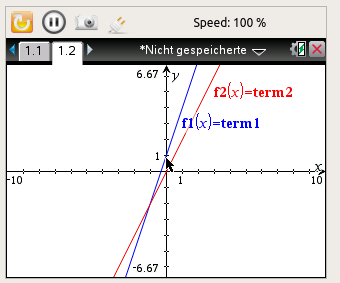
\includegraphics[width=6cm]{img/nspire_zwei_gleichungen.png}}
%  \end{center}
  Der Schnittpunkt der beiden Geraden zeigt die Variable $x$ (hier $-1$) und den Wert der beiden Terme (links bzw. rechts) des Gleichheitszeichens als Variable $y$ (hier $-2$) an.

\end{itemize}

\newpage
}

\subsection{Spezielle lineare Gleichungen}
\textbf{Typ A}\\

$$1+4x+2 = 5x - (x-3)$$
\TNT{6}{Alle Zahlen $x$ lösen die Gleichung!\vspace{14mm}}%% END TNT

\textbf{Typ B}\\

$$3x+8 = 5x-(2x-6)$$
\TNTeop{Keine Zahl $x$ löst die Gleichnug!\vspace{14mm}}%% END TNT


\subsection{Lösungsmenge}\index{Lösungsmenge}
  Die Zahlmenge, der gefundenen Lösungen einer Gleichung, nennen wir
  die Lösungsmenge und beschriften diese $\mathbb{L}$. Falls die gefundene
  Variable $x$ \zB{} den Wert $4$ hat, dann schreiben wir:
  $$\LoesungsRaumLang{\lx=\{4\}}$$
  Wenn eine Gleichung mehrere Lösungen hat (\zB $x=7$ und $x=-3$), so
  schreiben wir die Lösungsmenge in aufsteigender Form:
  $$\LoesungsRaumLang{\lx=\{-3; 7\}}$$
  Eine Gleichung ohne Lösung hat die leere Menge als Lösungsmenge und
  wir schreiben:
  $$\LoesungsRaumLang{\lx=\{\}}$$
  Falls alle Zahlen $x$ die Gleichung lösen, so schreiben wir:
  $$\LoesungsRaumLang{\lx=\mathbb{R}}$$

  

Die Lösungsmenge $\lx$ zur allgemeinen Grundform $ax+b=0$ lautet somit $$\LoesungsRaumLang{\lx=\left\{ \frac{-b}{a} \right\}.}$$

\begin{itemize}
  \item Im Spezialfall \textbf{Typ A} gilt $a=0$ und $b=0$. Hier kann ich für $x$ alles einsetzen und somit gilt $\lx=\mathbb{R}$.
  \item Im Spezialfall \textbf{Typ B} gilt $a=0$ und $b\ne 0$. Hier wird die Gleichung falsch, egal, was ich für $x$ einsetze; somit ist $\lx=\{\}$.
\end{itemize}



\subsection*{Aufgaben}
\AadBMTA{127ff}{2. a) f),  3. a) h), 4. f) und 6. a) d) e) f)}
%%\TALSAadBMTA{81}{223. a) b) e) 225. a) d) e) f) 227.a) b) c) 225. a) d) e) f) 229. a) 230. a) 231. d) 232. b)}

\olatLinkGESOKompendium{2.1.1.}{10}{1. bis 6.}

\newpage
